% Compile with XeLaTeX:  latexmk -xelatex -outdir=build main.tex
\documentclass[10pt, aspectratio=169]{beamer}

\usetheme{metropolis}
\metroset{progressbar=frametitle, numbering=fraction, block=fill, sectionpage=none}
\usepackage{appendixnumberbeamer}

\usepackage{booktabs}
\usepackage{amsmath, amssymb, mathtools, bm}
\usepackage{xspace}
\usepackage{tikz}
\usetikzlibrary{arrows.meta, positioning, shapes.geometric, calc, fit, backgrounds}
\usepackage{pgfplots}
\pgfplotsset{compat=1.18}
\usepackage{algpseudocodex}
\usepackage{algorithm}
\usepackage{multirow}

% ---- Bibliography (author-year) ----
\usepackage[style=authoryear, maxcitenames=2, maxbibnames=10, giveninits=true,
            uniquename=false, backend=bibtex, doi=false, isbn=false, url=false, eprint=true]{biblatex}
\addbibresource{refs.bib}
\renewcommand*{\bibfont}{\scriptsize}
\renewcommand*{\multicitedelim}{\addcomma\space}
\renewcommand*{\multinamedelim}{\addcomma\space}
\renewcommand*{\finalnamedelim}{\addspace\bibstring{and}\space}
\renewcommand*{\finentrypunct}{\addperiod}
\DeclareFieldFormat[article,misc]{title}{#1}
\DeclareFieldFormat{journaltitle}{\mkbibemph{#1}}
\renewbibmacro{in:}{}
\DeclareFieldFormat[article]{volume}{#1}
\DeclareFieldFormat[article]{number}{\mkbibparens{#1}}
\DeclareFieldFormat[article]{pages}{#1}
\DeclareFieldFormat{eprint:arxiv}{arXiv\addcolon\space #1}
\renewbibmacro*{volume+number+eid}{%
  \printfield{volume}%
  \printfield{number}%
  \setunit{\addcomma\space}%
  \printfield{eid}}
\setbeamertemplate{bibliography item}{}
\setbeamerfont{bibliography entry title}{series=\mdseries}
\setbeamertemplate{frametitle continuation}{}
\setbeamercolor{bibliography entry author}{fg=black!85}
\setbeamercolor{bibliography entry title}{fg=black!85}
\setbeamercolor{bibliography entry location}{fg=black!70}
\setbeamercolor{bibliography entry note}{fg=black!70}

% ---- Palette: restrained, journal-like ----
\definecolor{navy}{HTML}{1F3A5F}
\definecolor{slate}{HTML}{4A5A6A}
\definecolor{accent}{HTML}{B5462E}
\definecolor{lightbg}{HTML}{F2F4F7}
\definecolor{green2}{HTML}{3F7F5F}
\setbeamercolor{frametitle}{bg=navy, fg=white}
\setbeamercolor{progress bar}{fg=accent, bg=lightbg}
\setbeamercolor{title separator}{fg=accent}
\setbeamercolor{normal text}{fg=black!85}
\setbeamercolor{alerted text}{fg=accent}
\setbeamercolor{block title}{bg=navy!12, fg=navy}
\setbeamercolor{block body}{bg=lightbg}
\setbeamercolor{background canvas}{bg=white}
\setbeamertemplate{itemize item}{\color{navy}$\bullet$}
\setbeamertemplate{itemize subitem}{\color{slate}\scriptsize$\blacktriangleright$}

% ---- Tighter lists ----
\let\olditemize\itemize
\renewcommand{\itemize}{\olditemize\setlength{\itemsep}{0.35ex}\setlength{\parskip}{0pt}}
\usepackage{array}
\newcolumntype{L}[1]{>{\raggedright\arraybackslash}p{#1}}

% ---- Numbered captions for figures, tables and algorithms ----
\setbeamertemplate{caption}[numbered]
\setbeamertemplate{caption label separator}{.\ }
\setbeamerfont{caption}{size=\scriptsize}
\setbeamerfont{caption name}{size=\scriptsize, series=\bfseries}
\setbeamercolor{caption name}{fg=navy}
\usepackage{float}

% ---- Helpers ----
\newcommand{\E}{\mathbb{E}}
\newcommand{\where}{{\footnotesize\color{slate}where}}
\newcommand{\paperref}[1]{{\scriptsize\color{slate}\AtNextCitekey{\defcounter{maxnames}{99}}\fullcite{#1}\par}\vspace{0.6ex}}
\newcommand{\smallnote}[1]{{\footnotesize\color{slate}#1}}
\newcommand{\hl}[1]{\textcolor{accent}{#1}}
\newcommand{\key}[1]{\textcolor{accent}{\textbf{#1}}}
\tikzset{
  box/.style={draw=navy, fill=navy!6, rounded corners=2pt, align=center,
              font=\scriptsize, minimum height=0.95cm, text width=2.15cm, line width=0.5pt},
  boxacc/.style={box, draw=accent, fill=accent!7},
  arr/.style={-{Stealth[length=2mm]}, line width=0.6pt, color=slate},
}

\title{Term-Structure Signals for Commodity Calendar Spreads}
\subtitle{MTH 9897 Systematic Trading, Final Project (Project 7) \\ Proposal and Literature Review}
\author{Jiaheng Han \quad Tian Tian}
\institute{Baruch College, MFE Program}
\date{October 13, 2026}

\begin{document}

% =====================================================================
\maketitle

% =====================================================================
\section{Question}

\begin{frame}{Research Question and Setting}
\begin{columns}[T, onlytextwidth]
\begin{column}{0.56\textwidth}
\footnotesize
\begin{itemize}
  \item A calendar spread trades two maturities of the same commodity
  \[
    C_t = F(t,T_1) - F(t,T_2), \qquad T_1 < T_2
  \]
  \item Long the spread means long the near and short the far contract, with P\&L
        $\Pi_{t,t+h} = q\,M\,\Delta C_{t+h}$
  \item \where\ $F(t,T)$ is the price at date $t$ of the contract expiring at $T$, $q$ the
        number of spreads, $M$ the contract multiplier, and $\Delta C_{t+h} = C_{t+h}-C_t$
        on the same two contracts
  \item Research question: \key{does term-structure information $\bm{X_t}$ predict the spread change,
        net of rolls and costs?}
  \[
    \E_t\bigl[\Delta C_{t+h}\bigr] = f(X_t)
  \]
  \item \where\ $\E_t$ is the expectation given information at $t$, $h$ the holding horizon
        in days and $f$ an unknown forecasting function
\end{itemize}
\end{column}
\begin{column}{0.41\textwidth}
\begin{figure}
\centering
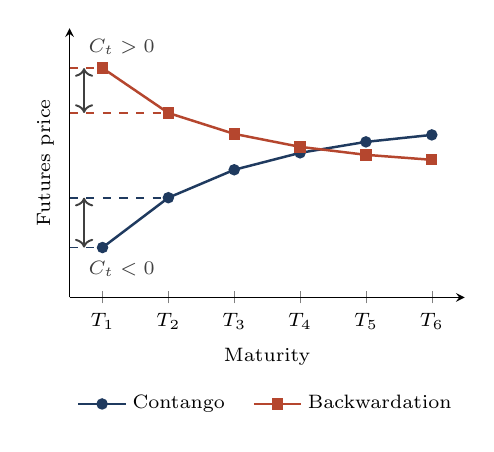
\begin{tikzpicture}
\begin{axis}[
  width=6.6cm, height=5.0cm,
  xlabel={\scriptsize Maturity}, ylabel={\scriptsize Futures price},
  xmin=0.5, xmax=6.5, ymin=57, ymax=84, clip=false,
  xtick={1,2,3,4,5,6}, xticklabels={$T_1$,$T_2$,$T_3$,$T_4$,$T_5$,$T_6$},
  ytick=\empty, tick label style={font=\scriptsize},
  axis lines=left, legend columns=2,
  legend style={font=\scriptsize, draw=none, at={(0.5,-0.32)}, anchor=north,
                /tikz/every even column/.append style={column sep=8pt}},
  every axis plot/.append style={line width=0.9pt, mark size=1.6pt}]
\addplot[color=navy, mark=*] coordinates {(1,62) (2,67) (3,69.8) (4,71.5) (5,72.6) (6,73.3)};
\addlegendentry{Contango}
\addplot[color=accent, mark=square*] coordinates {(1,80) (2,75.5) (3,73.4) (4,72.1) (5,71.3) (6,70.8)};
\addlegendentry{Backwardation}
% dashed guides from the price axis to F(t,T1) and F(t,T2), arrow left of T1
\draw[dashed, color=navy, line width=0.6pt]   (axis cs:0.5,62)   -- (axis cs:1,62);
\draw[dashed, color=navy, line width=0.6pt]   (axis cs:0.5,67)   -- (axis cs:2,67);
\draw[dashed, color=accent, line width=0.6pt] (axis cs:0.5,80)   -- (axis cs:1,80);
\draw[dashed, color=accent, line width=0.6pt] (axis cs:0.5,75.5) -- (axis cs:2,75.5);
\draw[<->, color=black!75, line width=0.7pt] (axis cs:0.72,62) -- (axis cs:0.72,67);
\node[font=\scriptsize, color=black!75, anchor=north west, inner sep=1pt] at (axis cs:0.74,61) {$C_t<0$};
\draw[<->, color=black!75, line width=0.7pt] (axis cs:0.72,75.5) -- (axis cs:0.72,80);
\node[font=\scriptsize, color=black!75, anchor=south west, inner sep=1pt] at (axis cs:0.74,81) {$C_t>0$};
\end{axis}
\end{tikzpicture}
\caption{Stylized futures curves on one date. Dashed lines mark $F(t,T_1)$ and $F(t,T_2)$, the arrow between them is the spread $C_t$.}
\end{figure}
\end{column}
\end{columns}
\end{frame}

% =====================================================================
\section{Literature}

% ---------------- Paschke et al. (2020) ------------------------------
\begin{frame}{Curve Momentum}
\paperref{paschke2020curve}
\begin{columns}[T, onlytextwidth]
\begin{column}{0.5\textwidth}
\footnotesize
\begin{itemize}
  \item Asks whether momentum exists within one futures curve rather than across commodities
  \item Return of nearby $i$ always uses the same contract, also on roll days
  \[
    R^{(i)}_{t+1} =
    \begin{cases}
      F^{(i)}_{t+1}/F^{(i)}_{t} - 1, & \text{no roll at } t\\[2pt]
      F^{(i)}_{t+1}/F^{(i+1)}_{t} - 1, & \text{roll at } t
    \end{cases}
  \]
  \item \where\ $F^{(i)}_t$ is the price of the $i$-th nearest contract at $t$ and
        $R^{(i)}_{t+1}$ its excess return from $t$ to $t+1$
  \item Signal is the past 12-month return of each nearby, \key{long the higher one, short the
        other}, held for one month
  \item CRB daily data, 22 commodities in 7 sectors, January 1986 to February 2015
\end{itemize}
\end{column}
\begin{column}{0.47\textwidth}
\begin{table}
\centering
\scriptsize
\setlength{\tabcolsep}{3pt}
\begin{tabular}{lcccc}
\toprule
 & Mean & $t$-stat & Gross SR & Net SR \\
\midrule
Energy      & 1.10 & (2.08) & 0.36 & \hl{$-0.11$} \\
Grains      & 2.37 & (3.87) & 0.78 & 0.65 \\
Meats       & 5.07 & (4.88) & 0.99 & 0.99 \\
Metals      & 0.12 & (0.66) & 0.13 & $-0.15$ \\
\midrule
Diversified & \textbf{1.76} & \textbf{(6.24)} & \textbf{1.28} & \textbf{0.93} \\
Long 2nd, short 1st & 1.49 & (4.54) & 1.03 & \\
\bottomrule
\end{tabular}
\caption{Curve momentum with a 12-month signal and 1-month holding, selected sectors.
Mean is the annualized excess return in percent, SR the Sharpe ratio, net of brokerage and one tick per trade.}
\end{table}
\vspace{-1ex}
\begin{itemize}\footnotesize
  \item Timing explains 57.75\% of the mean return, the rest is a static tilt
  \item \key{Energy turns negative after costs} because monthly expiries raise turnover
\end{itemize}
\end{column}
\end{columns}
\end{frame}

% ---------------- Lubnau and Todorova (2015) -------------------------
\begin{frame}{Mean Reversion with Dynamic Hedge Ratios}
\paperref{lubnau2015trading}
\begin{columns}[T, onlytextwidth]
\begin{column}{0.52\textwidth}
\footnotesize
\begin{itemize}
  \item Hedge ratio between near contract $A$ and far contract $B$ follows a state-space model
  \begin{align*}
    p_{A,t} &= \beta_{1,t} + \beta_{2,t}\,p_{B,t} + v_t\\
    \beta_{j,t} &= \beta_{j,t-1} + w_{j,t}, \qquad j = 1,2
  \end{align*}
  \item \where\ $p_{A,t}$, $p_{B,t}$ are settlement prices, $\beta_{1,t}$ an intercept,
        $\beta_{2,t}$ the hedge ratio, and $v_t$, $w_{j,t}$ Gaussian noises, filtered daily
        by the Kalman filter
  \item Trading signal on the hedged portfolio
  \[
    z_t = \frac{p_{H,t} - \mathrm{MA}_{L,t}}{\sigma_{L,t}}, \qquad p_{H,t} = p_{A,t} - \hat\beta_{2,t}\,p_{B,t}
  \]
  \item \where\ $p_{H,t}$ is the hedged portfolio value, $\mathrm{MA}_{L,t}$ and
        $\sigma_{L,t}$ its moving mean and standard deviation over $L \in \{20,50,100,200\}$ days
\end{itemize}
\end{column}
\begin{column}{0.45\textwidth}
\footnotesize
\begin{itemize}
  \item \key{Enter long when $\bm{z_t < -2}$ and short when $\bm{z_t > 2}$}, exit when $z_t$ returns to 0
  \item WTI, natural gas, heating oil and gasoline, front month against months 2 to 5, 1992 to 2013
  \item Cost of 0.1\% of price per trade, four trades per round turn
  \item \key{Sharpe ratios above 2} for most WTI and natural gas pairs, holding periods of 2 to 21 days
  \item Significance from 1{,}000 random-entry portfolios with matched trade counts
  \item Entries occur in both contango and backwardation
  \item \hl{Caveat}: a change in $\hat\beta_{2,t}$ moves $p_{H,t}$ without generating P\&L
\end{itemize}
\end{column}
\end{columns}
\end{frame}

% ---------------- Bianchi et al. (2023) ------------------------------
\begin{frame}{Nelson and Siegel Curve Dynamics}
\paperref{bianchi2023exploiting}
\begin{columns}[T, onlytextwidth]
\begin{column}{0.52\textwidth}
\footnotesize
\begin{itemize}
  \item Fits the \textcite{nelson1987parsimonious} curve each day to the nearest 4 contracts
  \begin{align*}
    F_t(M) = \beta_{L,t} &+ \beta_{S,t}\,\frac{1-e^{-\lambda_t M}}{\lambda_t M}\\
    &+ \beta_{C,t}\Bigl(\frac{1-e^{-\lambda_t M}}{\lambda_t M} - e^{-\lambda_t M}\Bigr) + \varepsilon_{t,M}
  \end{align*}
  \item \where\ $F_t(M)$ is the price of the contract with $M$ months to maturity,
        $\beta_{L,t}$, $\beta_{S,t}$, $\beta_{C,t}$ the level, slope and curvature factors,
        $\lambda_t$ the decay rate and $\varepsilon_{t,M}$ the fitting error
  \item Slope strategy: \key{long 1st and short 4th contract if $\bm{\Delta\beta_{S,t} > 0}$},
        reverse otherwise, held for one day, where $\Delta$ is the daily change
  \item 21 commodities, January 1992 to June 2019, average fit $R^2$ of 96.5\%
\end{itemize}
\end{column}
\begin{column}{0.45\textwidth}
\begin{figure}
\centering
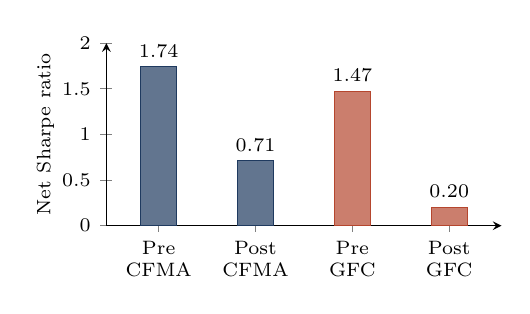
\begin{tikzpicture}
\begin{axis}[
  ybar, bar width=13pt, width=6.6cm, height=3.9cm, bar shift=0pt,
  ymin=0, ymax=2.0, ylabel={\scriptsize Net Sharpe ratio}, ylabel style={yshift=-4pt},
  symbolic x coords={PreCFMA, PostCFMA, PreGFC, PostGFC},
  xtick={PreCFMA, PostCFMA, PreGFC, PostGFC},
  xticklabels={Pre\\CFMA, Post\\CFMA, Pre\\GFC, Post\\GFC},
  tick label style={font=\scriptsize, align=center}, axis lines=left, enlarge x limits=0.18,
  nodes near coords={\pgfmathprintnumber[fixed, fixed zerofill, precision=2]{\pgfplotspointmeta}},
  nodes near coords style={font=\scriptsize}]
\addplot[fill=navy!70, draw=navy] coordinates {(PreCFMA,1.74) (PostCFMA,0.71)};
\addplot[fill=accent!70, draw=accent] coordinates {(PreGFC,1.47) (PostGFC,0.20)};
\end{axis}
\end{tikzpicture}
\caption{Net Sharpe ratio of the slope strategy before and after December 2000 (CFMA) and March 2009 (GFC).}
\end{figure}
\vspace{-1ex}
\begin{itemize}\footnotesize
  \item Gross Sharpe ratio 1.41, \key{net 0.44 to 1.04}
  \item Our sample starts in 2009, inside the weak regime
\end{itemize}
\end{column}
\end{columns}
\end{frame}

% ---------------- Synthesis ------------------------------------------
\begin{frame}{Summary of the Literature}
\begin{table}
\centering
\scriptsize
\setlength{\tabcolsep}{4pt}
\begin{tabular}{L{3.2cm}L{2.1cm}L{2.3cm}L{1.3cm}L{1.6cm}L{3.0cm}}
\toprule
Paper & Mechanism & Signal & Holding & Gross SR & Net of costs \\
\midrule
\textcite{paschke2020curve}      & Relative momentum   & 12-month return gap & 1 month      & 1.28           & 0.85 to 0.93, energy negative \\
\textcite{lubnau2015trading}     & Mean reversion      & Kalman $z$-score    & 2 to 21 days & above 2 (WTI)  & costs already included \\
\textcite{bianchi2023exploiting} & Factor continuation & Change in NS slope  & 1 day        & 1.41           & 0.44 to 1.04, decaying \\
\textcite{boons2019basis}        & Priced risk         & Basis-momentum      & 1 month      & about 0.9      & robust to estimated costs \\
\textcite{hong2026hierarchical}  & Learned prediction  & Graph neural network & 1 day       & daily IR 0.085 & not reported \\
\bottomrule
\end{tabular}
\caption{Five studies of term-structure trading. SR is the annualized Sharpe ratio, IR the information ratio.}
\end{table}
\begin{itemize}\footnotesize
  \item All signals come from the shape and recent dynamics of the futures curve
  \item Returns are small in level but have low volatility, so \key{costs and turnover decide profitability}
  \item Continuation and mean reversion coexist at different horizons
  \item Results are hard to compare because leg ratios, cost models and samples differ
  \item \key{Evidence after 2009 is thin}, which is exactly where our data lie
\end{itemize}
\end{frame}

% =====================================================================
\section{Proposed Approach}

\begin{frame}{Proposed Framework}
\begin{figure}
\centering
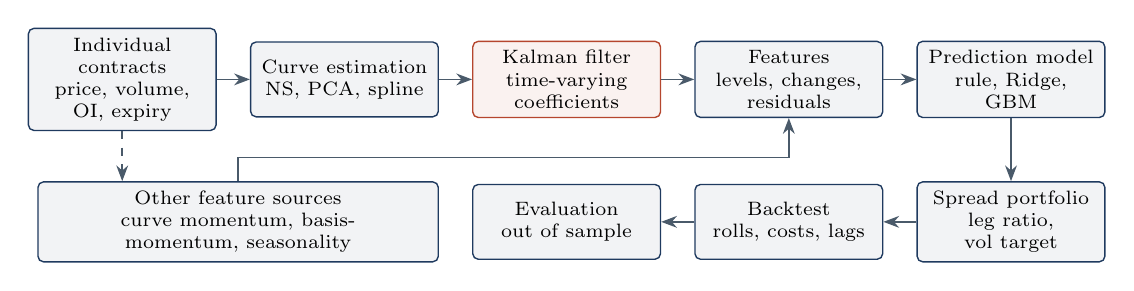
\begin{tikzpicture}[node distance=0.42cm and 0.42cm]
\node[box] (raw) {Individual contracts\\ price, volume, OI, expiry};
\node[box, right=of raw] (curve) {Curve estimation\\ NS, PCA, spline};
\node[boxacc, right=of curve] (kf) {Kalman filter\\ time-varying coefficients};
\node[box, right=of kf] (feat) {Features\\ levels, changes, residuals};
\node[box, right=of feat] (model) {Prediction model\\ rule, Ridge, GBM};
\node[box, below=0.8cm of model] (port) {Spread portfolio\\ leg ratio, vol target};
\node[box, left=of port] (bt) {Backtest\\ rolls, costs, lags};
\node[box, left=of bt] (eval) {Evaluation\\ out of sample};
\node[box, left=of eval, text width=4.85cm] (alt) {Other feature sources\\ curve momentum, basis-momentum, seasonality};
\draw[arr] (raw) -- (curve);
\draw[arr] (curve) -- (kf);
\draw[arr] (kf) -- (feat);
\draw[arr] (feat) -- (model);
\draw[arr] (model) -- (port);
\draw[arr] (port) -- (bt);
\draw[arr] (bt) -- (eval);
\draw[arr] (alt.north) -- ++(0,0.3) -| (feat.south);
\draw[arr, dashed] (raw.south) -- (alt.north -| raw.south);
\end{tikzpicture}
\caption{Research pipeline. \key{The Kalman filter turns daily curve fits into smooth state estimates that serve as features.}}
\end{figure}
\begin{columns}[T, onlytextwidth]
\begin{column}{0.48\textwidth}
\begin{itemize}\footnotesize
  \item Baselines: always long 2nd and short 1st, course Example 1, curve momentum,
        Kalman $z$-score, NS slope rule
  \item Every strategy is scaled to \key{the same volatility target} before comparison
\end{itemize}
\end{column}
\begin{column}{0.48\textwidth}
\begin{itemize}\footnotesize
  \item Metrics: out-of-sample $R^2$, net Sharpe ratio with Newey and West $t$-statistics, turnover with rolls
  \item 2009 to 2015 checks replication, \key{2016 onward is out of sample}
\end{itemize}
\end{column}
\end{columns}
\end{frame}

\begin{frame}{Model Specification}
\begin{columns}[T, onlytextwidth]
\begin{column}{0.5\textwidth}
\footnotesize
\begin{itemize}
  \item \key{Dynamic curve in state space}, following \textcite{diebold2006forecasting}
  \begin{align*}
    F_t(\tau_k) &= \bm\Lambda(\tau_k)^{\top}\bm\beta_t + \varepsilon_{t,k}\\
    \bm\beta_t &= \bm\mu + \bm\Phi\,(\bm\beta_{t-1}-\bm\mu) + \bm\eta_t
  \end{align*}
  \item \where\ $\tau_k$ is the time to maturity of contract $k$, $\bm\Lambda(\tau_k)$ the
        vector of NS loadings, $\bm\beta_t$ the level, slope and curvature states,
        $\bm\mu$ their long-run mean, $\bm\Phi$ the persistence matrix, and
        $\varepsilon_{t,k}$, $\bm\eta_t$ Gaussian errors
  \item Time-varying hedge relation between the two legs
  \[
    F_t(T_1) = \alpha_t + \gamma_t\,F_t(T_2) + v_t
  \]
  \item \where\ $\alpha_t$ and $\gamma_t$ follow random walks and $\gamma_t$ is the hedge ratio
\end{itemize}
\end{column}
\begin{column}{0.47\textwidth}
\footnotesize
\begin{itemize}
  \item Prediction target on \key{a fixed pair of contracts}
  \[
    Y_{t,h} = \frac{\Delta_h F(T_1) - \Delta_h F(T_2)}{\hat\sigma_t}, \qquad \hat Y_{t,h} = f_{\theta}(X_t)
  \]
  \item \where\ $\Delta_h F(T)$ is the price change from $t$ to $t+h$, $\hat\sigma_t$ the
        spread volatility estimated up to $t$, and $f_\theta$ a rule, Ridge or boosted trees with parameters $\theta$
  \item Features $X_t$ include $\hat{\bm\beta}_t$, $\Delta\hat{\bm\beta}_t$, $\hat\gamma_t$, the
        standardized Kalman innovation, the curve momentum gap, days to expiry and seasonality
  \item Position proportional to $\hat Y_{t,h}$, \key{set to zero when the forecast is below the
        round-trip cost}
  \item Walk-forward estimation, signal at the close of $t$, trade at $t+1$
\end{itemize}
\end{column}
\end{columns}
\end{frame}

% =====================================================================
\section{Data and Platform}

\begin{frame}{Data and Platform: QuantConnect US Futures}
\begin{columns}[T, onlytextwidth]
\begin{column}{0.5\textwidth}
\begin{table}
\centering
\scriptsize
\begin{tabular}{lL{4.4cm}}
\toprule
Provider   & AlgoSeek, hosted by QuantConnect \\
Coverage   & May 2009 to present \\
Universe   & 162 most liquid contracts \\
Exchanges  & CME, CBOT, NYMEX, COMEX, ICE, CFE \\
Resolution & Tick, second, minute, hour, daily \\
Fields     & Trade and quote bars, volume, open interest, expiry \\
Daily bar  & 12 AM to 12 AM ET, not the CME settlement \\
Access     & Free in the cloud, local download is paid \\
\bottomrule
\end{tabular}
\caption{QuantConnect US Futures dataset.}
\end{table}
\begin{itemize}\footnotesize
  \item Start with WTI crude (CL), first 4 to 6 contracts, then HO, RB, NG
  \item \key{Spreads use raw contract prices, never back-adjusted series}
\end{itemize}
\end{column}
\begin{column}{0.47\textwidth}
\footnotesize
\begin{itemize}
  \item[\textcolor{green2}{$+$}] True contract-level history with expiry and open interest
  \item[\textcolor{green2}{$+$}] Research notebooks and an event-driven backtester in one place
  \item[\textcolor{green2}{$+$}] Built-in fill, fee, slippage and margin models
  \item[\textcolor{green2}{$+$}] Intraday data available for execution studies
  \item[\textcolor{accent}{$-$}] \key{History starts in 2009}, after the strongest published regimes
  \item[\textcolor{accent}{$-$}] \key{Daily close is not the settlement price}, a problem for thin back months
  \item[\textcolor{accent}{$-$}] Raw data cannot be exported for free, which complicates reproducibility
  \item[\textcolor{accent}{$-$}] Cloud compute limits heavy model training
  \item Fallback: WRDS LSEG Datastream futures with settlement prices back to the 1970s
\end{itemize}
\end{column}
\end{columns}
\end{frame}

\begin{frame}{QuantConnect Architecture}
\begin{figure}
\centering
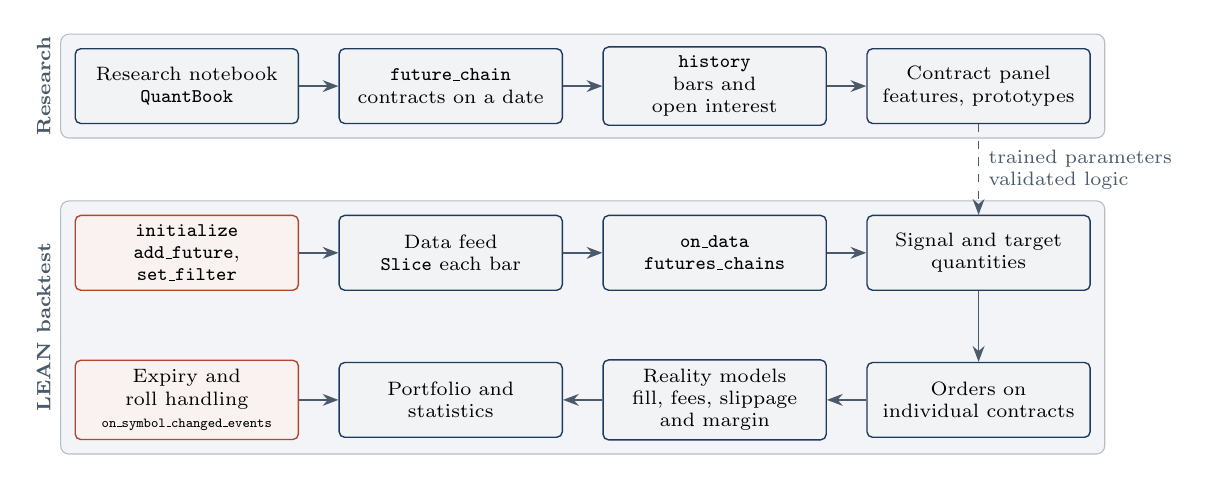
\begin{tikzpicture}[node distance=0.36cm and 0.5cm]
\node[box, text width=2.6cm] (qb) {Research notebook\\ \texttt{QuantBook}};
\node[box, right=of qb, text width=2.6cm] (chain) {\texttt{future\_chain}\\ contracts on a date};
\node[box, right=of chain, text width=2.6cm] (hist) {\texttt{history}\\ bars and open interest};
\node[box, right=of hist, text width=2.6cm] (panel) {Contract panel\\ features, prototypes};
\draw[arr] (qb) -- (chain);
\draw[arr] (chain) -- (hist);
\draw[arr] (hist) -- (panel);
\node[boxacc, below=1.15cm of qb, text width=2.6cm] (init) {\texttt{initialize}\\ \texttt{add\_future}, \texttt{set\_filter}};
\node[box, right=of init, text width=2.6cm] (slice) {Data feed\\ \texttt{Slice} each bar};
\node[box, right=of slice, text width=2.6cm] (ondata) {\texttt{on\_data}\\ \texttt{futures\_chains}};
\node[box, right=of ondata, text width=2.6cm] (sig) {Signal and target\\ quantities};
\node[box, below=0.9cm of sig, text width=2.6cm] (orders) {Orders on\\ individual contracts};
\node[box, left=of orders, text width=2.6cm] (models) {Reality models\\ fill, fees, slippage\\ and margin};
\node[box, left=of models, text width=2.6cm] (pf) {Portfolio and statistics};
\node[boxacc, left=of pf, text width=2.6cm] (roll) {Expiry and roll handling\\ {\tiny\texttt{on\_symbol\_changed\_events}}};
\draw[arr] (init) -- (slice);
\draw[arr] (slice) -- (ondata);
\draw[arr] (ondata) -- (sig);
\draw[arr] (sig) -- (orders);
\draw[arr] (orders) -- (models);
\draw[arr] (models) -- (pf);
\draw[arr] (roll) -- (pf);
\draw[arr, dashed] (panel.south) -- node[right, font=\scriptsize, color=slate, align=left]{trained parameters\\ validated logic} (sig.north);
\begin{scope}[on background layer]
\node[fit=(qb)(panel), draw=slate!40, fill=lightbg, rounded corners=3pt, inner sep=5pt,
      label={[font=\scriptsize\bfseries, color=slate]west:\rotatebox{90}{Research}}] {};
\node[fit=(init)(sig)(orders)(roll), draw=slate!40, fill=lightbg, rounded corners=3pt, inner sep=5pt,
      label={[font=\scriptsize\bfseries, color=slate]west:\rotatebox{90}{LEAN backtest}}] {};
\end{scope}
\end{tikzpicture}
\caption{Research environment (top) and event-driven LEAN backtest (bottom). Signals use the
continuous symbol, \key{orders target individual contracts with raw prices}.}
\end{figure}
\end{frame}

\begin{frame}[fragile]{Algorithm Sketch for a Spread Strategy}
\begin{columns}[T, onlytextwidth]
\begin{column}{0.6\textwidth}
\begin{algorithm}[H]
\caption{Daily calendar spread strategy in LEAN}
\scriptsize
\begin{algorithmic}[1]
\Procedure{Initialize}{}
  \State \texttt{fut} $\gets$ \texttt{add\_future(CL, DAILY, RAW)}
  \State \texttt{fut.set\_filter(0, 182)} \Comment{contracts within 6 months}
  \State set fee, slippage and margin models
  \State schedule \Call{Rebalance}{} after the daily close
\EndProcedure
\Procedure{Rebalance}{chain}
  \State sort chain by expiry, drop contracts within $D$ days of expiry
  \State $(T_1, T_2) \gets$ first two remaining contracts
  \State update curve fit and Kalman states with today's prices
  \State $X_t \gets$ features, \ $\hat Y \gets f_{\theta}(X_t)$
  \If{forecast exceeds the cost threshold}
    \State hold $+q_1$ contracts of $T_1$ and $-q_2$ contracts of $T_2$
  \Else
    \State liquidate the spread
  \EndIf
\EndProcedure
\Procedure{OnSecuritiesChanged}{}
  \State close legs that left the filter, reopen on the new pair
\EndProcedure
\end{algorithmic}
\end{algorithm}
\end{column}
\begin{column}{0.37\textwidth}
\begin{itemize}\footnotesize
  \item $T_1$ and $T_2$ are the near and far contracts, $X_t$ and $f_\theta$ as in the model specification
  \item $D$ is the safety margin in days before expiry, $q_1$ and $q_2$ the leg sizes
  \item \key{Signals use the contract panel}, not the stitched continuous series
  \item Both legs are chosen by expiry rank, so \key{they roll together}
  \item One scheduled event per day avoids look-ahead from intraday bars
  \item Model parameters are trained in research and refit on a fixed calendar
\end{itemize}
\end{column}
\end{columns}
\end{frame}

% =====================================================================
\section{Challenges}

\begin{frame}{Anticipated Difficulties and Open Questions}
\begin{columns}[T, onlytextwidth]
\begin{column}{0.48\textwidth}
\begin{itemize}\footnotesize
  \item \key{Contract panel and rolls}: rebuild the curve from historical chains and keep
        P\&L on the held contracts for both legs
  \item \key{Noisy curve fits}: only 4 to 6 contracts per day, so NS factors and their daily
        changes are fragile without filtering
  \item \key{Costs}: spread returns are small, and no daily bid and ask history is available
  \item \key{Short sample}: data start in 2009, when published effects are already weaker
\end{itemize}
\end{column}
\begin{column}{0.48\textwidth}
\begin{block}{Questions for discussion}
\begin{itemize}\footnotesize
  \item Is the proposed framework reasonable: Kalman-filtered curve states as features,
        a forecast of the standardized spread change, and positions scaled by the forecast?
  \item Is it sound to replicate the coefficient-based features of the papers, namely the NS
        slope and curvature changes, the Kalman hedge ratio and the momentum gap, on post-2009
        QuantConnect data and use them as inputs rather than as standalone rules?
\end{itemize}
\end{block}
\end{column}
\end{columns}
\end{frame}

% =====================================================================
\begin{frame}[standout]
  Thank you
  \vspace{1.5ex}

  {\normalsize Suggestions and questions are welcome}
\end{frame}

% =====================================================================
\appendix

\begin{frame}[allowframebreaks]{References}
\nocite{*}
\printbibliography[heading=none]
\end{frame}

\end{document}
